\subsubsection{Resultater}
Fra app'ens hovedmenu kan brugeren tilgå sine resultater. Hvis dette tilgås henter systemet resultater vedrørende brugeren i databasen. Systemet viser grafisk udviklingen af brugerens træning på uge- og månedsbasis. Herefter er der mulighed for at få vist kalender og belønninger. Aktivitetsdiagrammet over resultater fremgår af \autoref{fig:resultater}.

\\begin{figure} [H]
\centering
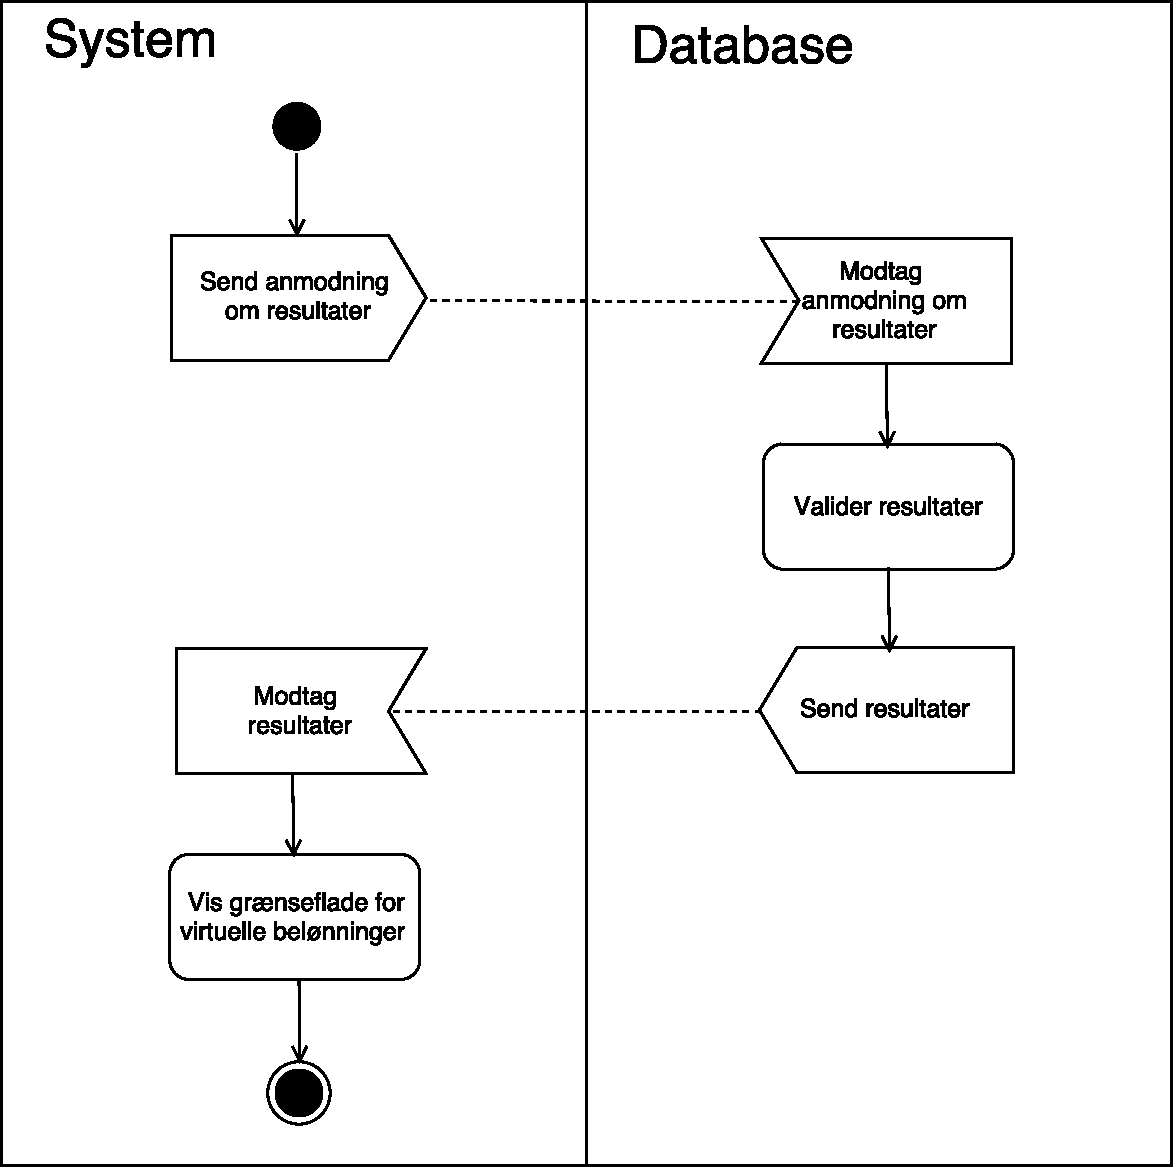
\includegraphics[width=0.9\textwidth]{figures/aktivitetsdiagram/Resultater}
\caption{Aktivitetsdiagram over resultater.}
\label{fig:resultater}
\end{figure}

\noindent
I kalenderen kan brugeren få et overblik over, hvilke dage der er udført træning samt de resultater der er opnået de enkelte dage. I belønninger kan brugerne se, hvilke virtuelle belønninger de og andre brugere har opnået i forbindelse med fuldført træning. Belønningerne varierer afhængig af træningsform. Inden for hver træningsform, jf. \autoref{sec:traening}, kan der opnås pokaler inden for forskellige kategorier. Disse kategorier fremgår af \autoref{tab:beloenninger}.

\begin{figure} [H]
\centering
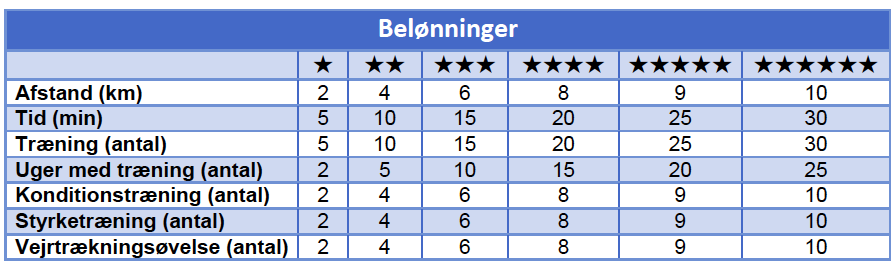
\includegraphics[width=0.9\textwidth]{figures/aktivitetsdiagram/beloeninnger}
\caption{Belønninger opnået ved træning.}
\label{tab:beloenninger}
\end{figure}
 

